%\documentclass{beamer}

\documentclass[10pt]{beamer} 
\usetheme[pageofpages=of,% String used between the current page and the
          % total page count.
          alternativetitlepage=true,% Use the fancy title page.
          %titlepagelogo=coca,% Logo for the first page.
          titleline=true
          ]{Torino}
%\usetheme{Frankfurt}
\usecolortheme{chameleon}

\usepackage{graphicx,hyperref,url}
\usepackage[utf8]{inputenc}
\usepackage[T1]{fontenc}
\usepackage[portuges,brazilian]{babel}
%%%\usepackage{wrapfig}
\usepackage{caption}
\usepackage{subfigure}
%\usepackage{subcaption}
\usepackage{latexsym}
\usepackage{amssymb, amsmath}
\usepackage{multicol}
\usepackage{pifont}%,bbding}%%,dingbat} %%% ver manual de simbolos
\usepackage[final]{listings}
\usepackage{comment}


\definecolor{azulclaro}{rgb}{0.9,0.9,0.9}
\definecolor{mygreen}{rgb}{0,0.6,0}
\definecolor{mygray}{rgb}{0.5,0.5,0.5}
\definecolor{mymauve}{rgb}{0.58,0,0.82}
\definecolor{darkgray}{rgb}{.4,.4,.4}
\definecolor{purple}{rgb}{0.65, 0.12, 0.82}

\newcommand{\minizinc}{MiniZinc}

\lstset{ 
  %  label={pgm_ex01},
    backgroundcolor=\color{azulclaro}, 
    language=erlang, %%Miranda,%%Perl,%%%Python, %%Mercury,
    showstringspaces=false,
    basicstyle=\bf\scriptsize\ttfamily,
%%      basicstyle= \footnotesize %%% TESTAR
%%      keywordstyle=\bfseries\color{green!40!black},
    keywordstyle=\textbf{\color{mygreen}}, 
    otherkeywords={*, \%, array, constraint, solve, output,  show, "/\", satisfy, set, of, if, then, elseif, float, search},
%%  keywordstyle=\color{blue},       % keyword style
%%    commentstyle=\itshape\color{purple!40!black},
      commentstyle=\color{orange},    % comment style
      identifierstyle=\color{blue},
      stringstyle=\color{orange},
      stringstyle=\color{mymauve},
      numbers=left,  % where to put the line-numbers; possible values are (none, left, right)
      numbersep=5pt,   % how far the line-numbers are from the code
      numberstyle=\tiny\color{magenta},
      keepspaces=true      
    % %caption={LEGENDA no source PASCAL ficou OK},
}


\graphicspath{{/home/ccs/Dropbox/figs_genericas/}{figuras/}{/home/ccs/Dropbox/CCS/picat}}
\DeclareGraphicsExtensions{.pdf,.png,.jpg}
%Global Background must be put in preamble
%\usebackgroundtemplate{\includegraphics[width=\paperwidth]{amarelinho.pdf}}
%%% \begin{frame}[allowframebreaks=0.8]

% The log drawn in the upper right corner.

%\logo{\centering
%\includegraphics[height=0.050\paperheight]{figuras/logo_SBPO_Peixe.png}
%%\hspace{9.6cm}
%\includegraphics[height=0.027\paperheight]{figuras/logo_udesc_horizontal.jpg}


%%%%%%%%%%%%%%%%%%%%%%%%%%%%%%%%%%%%%%%%%%%%%%%%%%%%%%%%%%%%%%%%%%%%%


\title[Picat]{\fontsize{20}{30}\selectfont \textcolor{black}{PICAT: uma Linguagem Multiparadigma}}

\author[Battisti \& PV]{Claudio Cesar de Sá, Rogério Eduardo da Silva,
    João Herique Faes Battisti, Paulo Victor de Aguiar\\\medskip
    {\small \url{joaobattisti@gmail.com}} \\ 
    {\small \url{pavaguiar@gmail.com}}\\
     {\small \url{claudio.sa@udesc.br}}}

\institute[UDESC]{
    Departamento de Ci\^encia da Computa\c{c}\~ao \\
    Centro de Ci\^encias e Tecnol\'ogias\\
Universidade do Estado de Santa Catarina}

%%%%%%%%%%%%%%%%%%%%%%%%%%%%%%%%%%%%%%%%%%%%%%%%%%%%%%%%%%%%%%%%%%%%%

\begin{document}

\begin{frame}
    \titlepage
\end{frame}

%%%%%%%%%%%%%%%%%%%%%%%%%%%%%%%%%%%%%%%%%%%%%%%%%%%%%%%%%%%%%%%%%%%%%

\begin{frame}[fragile]
\frametitle{Sumário}
\tableofcontents
\end{frame}

\section{Introdução}
\begin{frame}

    \frametitle{Histórico}

    \begin{itemize}
      \item Criada em 2013 por Neng-Fa Zhou e Jonathan Fruhman.
      \item Utilizou o B-Prolog como base de implementação, e ambas utilizam 
      a  programação em lógica baseada em regras de predicativas>
      \item Picat 0.1 – Teve seu lançamento em Maio de 2013.
      \item Picat 1.0 – Foi lançada Abril de 2015.
      \item Sua atual versão é a 2.0 (\today)
    \end{itemize}
\end{frame}

%%%%%%%%%%%%%%%%%%%%%%%%%%%%%%%%%%%%%%%%%%%%%%%%%%%%%%%%%%%%%%%%%%%%%

%\section{Isso é outra seção}
\begin{frame}
    \frametitle{Picat é Multiparadigma}
    \begin{itemize}
      \item Imperativo -- procedural
      \item Funcional
      \item \underline{Lógico}
    %  \item 
    \end{itemize}
\end{frame}

%%%%%%%%%%%%%%%%%%%%%%%%%%%%%%%%%%%%%%%%%%%%%%%%%%%%%%%%%%%%%%%%%%%%%

\begin{frame}
    \frametitle{Linguagem Multiparadigma}
    Motivo de existencia dos paradigmas?
    \begin{itemize}
      \item Sintaxe $\Rightarrow $ elegância do código%%Velocidade de implementação
      \item Velocidade de execução
      \item Portabilidade
    \end{itemize}
\end{frame}

%%%%%%%%%%%%%%%%%%%%%%%%%%%%%%%%%%%%%%%%%%%%%%%%%%%%%%%%%%%%%%%%%%%%%

\begin{frame}
    \frametitle{Linguagem Picat}
    \begin{itemize}
      \item Terminologia: segue as bases teóricas da linguagem Prolog.
    
      \item Na \textbf{l}ógica de \textbf{p}rimeira-\textbf{o}rdem (LPO) os objetos são chamados por \textbf{termos}.
      
      \item O destaque de Picat é a sua natureza declarativa, funcional, tipagem dinâmica, e sintaxe \textit{açucarada}
      
      \item \texttt{PICAT} é um anacrônico onde cada letra representa uma característica  de sua funcionalidade (operacionalidade).
    
    \end{itemize}
\end{frame}

%%%%%%%%%%%%%%%%%%%%%%%%%%%%%%%%%%%%%%%%%%%%%%%%%%%%%%%%%%%%%%%%%%%%%

\section{Características}
\begin{frame}
    \frametitle{Características: \textcolor{red}{P}-I-C-A-T}
 
 \textit{Pattern-matching}:\\ 
 \begin{itemize}
  \item     Utiliza o conceito de casamento padrão. 
  \item    Um predicado define uma relação entre objetos n-ários
  \item     Uma função é um predicado especial que sempre retorna uma única resposta. 
  \item     Ambos são definidos com regras de Picat, e seus predicados e funções seguem as regras de \textit{casamento-de-padrões}.

\end{itemize}

\end{frame}

%%%%%%%%%%%%%%%%%%%%%%%%%%%%%%%%%%%%%%%%%%%%%%%%%%%%%%%%%%%%%%%%%%%%%

\begin{frame}
    \frametitle{Características: P-\textcolor{red}{I}-C-A-T}
    \textit{Intuitive}:\\ 
 \begin{itemize}
 
 \item     O Picat oferece atribuições e laços de repetições para a programação dos dias de hoje. 
 \item         Uma variável atribuída  imita  variáveis lógicas, alterado seu valor seguindo o estado da computação. 
 \item        As atribuições são úteis para associar os termos, bem como utilizadas nas estruturas de laços repetitivos. 
    
 \end{itemize}
    
    
\end{frame}

%%%%%%%%%%%%%%%%%%%%%%%%%%%%%%%%%%%%%%%%%%%%%%%%%%%%%%%%%%%%%%%%%%%%%

\begin{frame}
    \frametitle{Características: P-I-\textcolor{red}{C}-A-T}
    \textit{Constraints}:\\ 
\begin{itemize}
      \item   Picat suporta a programação por restrições. 
 
  \item  Dado um conjunto de variáveis, 
    cada uma possui um domínio de valores possíveis e restrições para limitar os valores a serem atribuídos nas variáveis. 
 
 \item    O objetivo é atribuir os valores que satisfaçam todas as restrições. 

    \end{itemize}
    \end{frame}

%%%%%%%%%%%%%%%%%%%%%%%%%%%%%%%%%%%%%%%%%%%%%%%%%%%%%%%%%%%%%%%%%%%%%

\begin{frame}
    \frametitle{Características: P-I-C-\textcolor{red}{A}-T}
    \textit{Actors}: \textcolor{red}{ \textbf{REFAZER em breve  ...}}
  \begin{itemize}
      \item   Atores são chamadas orientadas à eventos.
		\item Em Picat, as regras de ação descrevem comportamentos dos atores.
\item 		Um ator recebe um objeto e dispara uma ação. 
\item 		Os eventos são postados via canais de mensagem e um ator pode ser conectado há um canal, verificar e/ou processar seus eventos postados no canal.

    \end{itemize}   
\end{frame}

%%%%%%%%%%%%%%%%%%%%%%%%%%%%%%%%%%%%%%%%%%%%%%%%%%%%%%%%%%%%%%%%%%%%%

\begin{frame}
    \frametitle{Características: P-I-C-A-\textcolor{red}{T}}
    \textit{Tabling}:
    \begin{itemize}
      \item     Considerando que operações entre variáveis podem ser armazenadas parcialmente em uma tabela na memória, permitindo que um programa acesse valores já calculados.
	\item 	Assim, evita-se a repetição de operações já realizadas.
	\item 	Com esta técnica de \textit{memoization}, o Picat oferece soluções imediatas para problemas de programação dinâmica.
    \end{itemize}
\end{frame}

%%%%%%%%%%%%%%%%%%%%%%%%%%%%%%%%%%%%%%%%%%%%%%%%%%%%%%%%%%%%%%%%%%%%%

\begin{frame}
    \frametitle{Comparações}
    \begin{table}[!bh]
\centering
\caption{Comparativo entre algumas linguagens: \url{https://rosettacode.org/wiki/Language_Comparison_Table}}
\label{tabela_ling_refs}
{\tiny
%%%\begin{tabular}{c|c|c|c|c|c|c}\hline \hline
%\begin{tabular}{C{2cm}|C{1.4cm}|C{1.4cm}|C{1.4cm}|C{1.4cm}|C{1.4cm}|C{1.4cm}}\hline \hline
\begin{tabular}{p{2cm}|p{1cm}|p{1cm}|p{1cm}|p{1cm}|p{1cm}}\hline \hline
      &\textbf{C}  &  \textbf{Haskell} &  \textbf{Java} &  \textbf{Prolog} &  \textbf{P.I.C.A.T}\\ \hline \hline
	    
Paradigma(s)	                        & procedural                                    & funcional                               & orientado à objetos   &  lógico                                             & multi-paradigma \\
\hline 

Tipagem	        & fraca                                         & forte                                   & forte                  &  fraca                                                         & fraca \\
\hline 

Verificação de tipos	                & estático                                      & estático                                & estático                              & dinâmico                                   & dinâmico \\

\hline  
Possui segurança?	                & não                                             & sim                                      & sim                                            & não                                          & sim\\

\hline  
Possui coletor de lixo?	                        & não                                                                        & sim                 &  sim                  & sim                                     & sim \\

\hline  
Passagem de parâmetros	                &  valor & -                                       &  valor                                     &  valor & casamento \\

\hline   
Legibilidade	  & baixa   & média     & média &  média       & boa \\


\hline 
\hline
\end{tabular} 
}

\end{table}
\end{frame}

%%%%%%%%%%%%%%%%%%%%%%%%%%%%%%%%%%%%%%%%%%%%%%%%%%%%%%%%%%%%%%%%%%%%%

\begin{frame}
    \frametitle{Usos}
    A linguagem Picat pode ser utilizada para diversas funções:
    \begin{itemize}
     \item Acadêmica
     \item Industrial
     \item Pesquisas
    \end{itemize}
\end{frame}


%%%%%%%%%%%%%%%%%%%%%%%%%%%%%%%%%%%%%%%%%%%%%%%%%%%%%%%%%%%%%%%%%%%%%

\begin{frame}
    \frametitle{Sistema de Programação}
    \begin{itemize}
     \item Picat é uma linguagem de multiplataforma, disponível em qualquer arquitetura de processamento e também de sistema operacional
     \item Utiliza a extensão .pi em seus arquivos de código fonte. 
     \item Existem 2 modos de utilização do Picat: Modo linha de comando e Modo Interativo. 
    \end{itemize}
\end{frame}

%%%%%%%%%%%%%%%%%%%%%%%%%%%%%%%%%%%%%%%%%%%%%%%%%%%%%%%%%%%%%%%%%%%%%

\begin{frame}
    \frametitle{Vantagens}
    \begin{itemize}
     \item Enfatiza uma visão moderna e controlável em seu mecanismo de backtracking.
     \item Clareza em construir regras declarativas.
     \item Funções disponíveis numa sintaxe análoga a Haskell com um ambiente de programação análogo ao Python.
     \item Biblioteca é organizada em módulo a exemplo de Haskell e Python. 
    \end{itemize}
\end{frame}

%%%%%%%%%%%%%%%%%%%%%%%%%%%%%%%%%%%%%%%%%%%%%%%%%%%%%%%%%%%%%%%%%%%%%

\begin{frame}
    \frametitle{Desvantagens}
    \begin{itemize}
     \item Manteve as letras maiúsculas para variáveis, como feito no B-Prolog.
     \item A geração de um código executável ainda não é puro, ela ainda se encontra em desenvolvimento
     \item As estruturas de repetição, comparadas com outras imperativas, ficam com uma sintaxe diferente. 
    \end{itemize}
\end{frame}

%%%%%%%%%%%%%%%%%%%%%%%%%%%%%%%%%%%%%%%%%%%%%%%%%%%%%%%%%%%%%%%%%%%%%

\section{Tipos de Dados}
\begin{frame}
\frametitle{Tipos de Dados}
\begin{figure}[!ht]
\centering
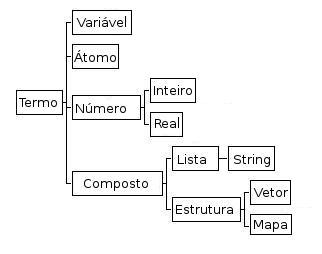
\includegraphics[width=.6\textwidth]{figures/tipos_dados_picat_traduzido.jpg}
\caption{Hierarquia dos Tipos de dados}
\label{Hiera}
\end{figure}
\end{frame}

%%%%%%%%%%%%%%%%%%%%%%%%%%%%%%%%%%%%%%%%%%%%%%%%%%%%%%%%%%%%%%%%%%%%%

\subsection{Variáveis}
\begin{frame}
    \frametitle{Variável}
    \begin{itemize}
     \item As variáveis em Picat são similares as variáveis das matemática, pois ambas guardam valores. 
	   Diferentemente das linguagens imperativas, as variáveis em Picat não possuem um endereço simbólico na memória do computador.
     \item Quando uma variável ainda não foi instanciada com um valor, ela fica em um estado livre. 
	   Uma vez quando for instanciada com um valor, ela terá a mesma identidade como se fosse um valor até que ela seja liberada de novo.
    \end{itemize}
\end{frame}

%%%%%%%%%%%%%%%%%%%%%%%%%%%%%%%%%%%%%%%%%%%%%%%%%%%%%%%%%%%%%%%%%%%%%
\subsection{Átomos}
\begin{frame}
    \frametitle{Átomos}
    \begin{itemize}
     \item Um átomo é uma constante simbólica e seu nome pode ser representado tanto com aspas simples ou sem. 
     \item Um átomo não pode ultrapassar uma linha de comando e seu nome tem um limite de mil caracteres. 
    
    Ex: x, x\_1, ’a’, ’b1’
    \end{itemize}
\end{frame}

%%%%%%%%%%%%%%%%%%%%%%%%%%%%%%%%%%%%%%%%%%%%%%%%%%%%%%%%%%%%%%%%%%%%%
\subsection{Números}
\begin{frame}
    \frametitle{Número}
    \begin{itemize}
     \item Um número é um átomo inteiro ou real. Um número inteiro pode ser representado na forma decimal, binária, octal ou hexadecimal. 
     \item Já o número real usa o ponto no lugar da virgula para separar os valores depois de zero como: 3.1415.
    \end{itemize}
\end{frame}

%%%%%%%%%%%%%%%%%%%%%%%%%%%%%%%%%%%%%%%%%%%%%%%%%%%%%%%%%%%%%%%%%%%%%

\begin{frame}
    \frametitle{Número}
    \texttt{Picat> A = 5, B = 7, number(A), number(B),
    max(A, B) = Maximo, min(A, B) = Minimo.}\\
  
    \texttt{A = 5}\\
    \texttt{B = 7}\\
    \texttt{Maximo = 7}\\
    \texttt{Minimo = 5}\\
    \texttt{yes.}
\end{frame}

%%%%%%%%%%%%%%%%%%%%%%%%%%%%%%%%%%%%%%%%%%%%%%%%%%%%%%%%%%%%%%%%%%%%%

\subsection{Termos Compostos}
\begin{frame}
    \frametitle{Termos Compostos}
    Um termo composto se divide entre listas,  estruturas e outros tipos compostos derivado destes são: 
    \textit{strings}, vetores e mapas. Entretanto, ambos tem seus elementos acessados via casamento de padrões de fatos, predicados e funções.
\end{frame}

%%%%%%%%%%%%%%%%%%%%%%%%%%%%%%%%%%%%%%%%%%%%%%%%%%%%%%%%%%%%%%%%%%%%%
\subsection{Listas}
\begin{frame}
    \frametitle{Listas}
    A forma de uma lista reúne um conjunto de termos e os coloca dentro de colchetes: [t1; t2; :::; tn]. Veja o exemplo:
\end{frame}

%%%%%%%%%%%%%%%%%%%%%%%%%%%%%%%%%%%%%%%%%%%%%%%%%%%%%%%%%%%%%%%%%%%%%

\begin{frame}
    \frametitle{Listas}
    \texttt{Picat> A=[1,2,3], list(A), length(A)=L\_A, B= [4,5,6], list(B),}\\
    \texttt{length(B) = L\_B, A ++ B = C, list(C), length(C) = L\_C.}\\

    \texttt{A = [1,2,3]}\\
    \texttt{L\_A = 3}\\
    \texttt{B = [4,5,6]}\\
    \texttt{L\_B = 3}\\
    \texttt{C = [1,2,3,4,5,6]}\\
    \texttt{L\_C = 6}\\
    \texttt{yes.}
\end{frame}

%%%%%%%%%%%%%%%%%%%%%%%%%%%%%%%%%%%%%%%%%%%%%%%%%%%%%%%%%%%%%%%%%%%%%
\subsection{Estruturas}
\begin{frame}
    \frametitle{Estruturas}
    A forma de uma estrutura é definida como \$s(t1, t2, ..., tn),onde s é um átomo e \$ é usado para diferenciar uma função. 
    Seus principais elementos são o nome da estrutura que é o átomo que fica na frente e a aridade (número de argumentos do predicado). 
    Veja o exemplo:
\end{frame}

%%%%%%%%%%%%%%%%%%%%%%%%%%%%%%%%%%%%%%%%%%%%%%%%%%%%%%%%%%%%%%%%%%%%%

\begin{frame}
    \frametitle{Estruturas}
    \texttt{Picat> N = \$nome(1,2,3,4,5), struct(N), arity(N) = Aridade,}\\
    \texttt{to\_list(N) = Lista.}\\

    \texttt{N = nome(1,2,3,4,5)}\\
    \texttt{Aridade = 5}\\
    \texttt{Lista = [1,2,3,4,5]}\\
    \texttt{yes.}
\end{frame}

%%%%%%%%%%%%%%%%%%%%%%%%%%%%%%%%%%%%%%%%%%%%%%%%%%%%%%%%%%%%%%%%%%%%%

\begin{frame}
    \frametitle{Estruturas}
    \texttt{Picat> N = \$(1,2,3,4,5), struct(N), arity(N) = Aridade,}\\
    \texttt{to\_list(N) = Lista.}\\

    \texttt{N = (1,2,3,4,5)}\\
    \texttt{Aridade = 2}\\
    \texttt{Lista = [1,(2,3,4,5)]}\\
    \texttt{yes.}
\end{frame}

%%%%%%%%%%%%%%%%%%%%%%%%%%%%%%%%%%%%%%%%%%%%%%%%%%%%%%%%%%%%%%%%%%%%%

\section{Exemplos}
\begin{frame}
    \frametitle{Exemplos}
    \begin{figure}[!ht]
    \centering
    
\includegraphics[width=.6\textwidth]{figures/exercicio.jpg}
    %\caption{Hierarquia dos Tipos de dados}
    %\label{Hiera}
    \end{figure}
\end{frame}

%%%%%%%%%%%%%%%%%%%%%%%%%%%%%%%%%%%%%%%%%%%%%%%%%%%%%%%%%%%%%%%%%%%%%

\begin{frame}
    \frametitle{Atribuição}
     \texttt{Picat> X := 7, X := X + 7, X := X + 7.}\\
     \texttt{X = 21}
\end{frame}

%%%%%%%%%%%%%%%%%%%%%%%%%%%%%%%%%%%%%%%%%%%%%%%%%%%%%%%%%%%%%%%%%%%%%

\begin{frame}
    \frametitle{Estruturas de Controle}
     \texttt{ex1 =>}\\
     \texttt{X:=3, Y:=4,}\\
     \texttt{if(X >= Y)}\\
     \texttt{then printf("\%d", X)}\\
     \texttt{else printf("\%d", Y)}\\
     \texttt{end.}
\end{frame}

%%%%%%%%%%%%%%%%%%%%%%%%%%%%%%%%%%%%%%%%%%%%%%%%%%%%%%%%%%%%%%%%%%%%%

%%%%%%%%%%%%%%%%%%%%%%%%%%%%%%%%%%%%%%%%%%%%%%%%%%%%%%%%%%%%%%%%%%%%%
\subsection{Entradas e Sa\'idas}
\begin{frame}
    \frametitle{Entradas e Saídas}
    \texttt{main =>}\\
    \texttt{printf("Digite dois números: "),}\\
    \texttt{N$\_real01 = read\_$real(),}\\
    \texttt{N$\_real02 = read\_$real(),}\\
    \texttt{Media = (N$\_real01+N\_real$02)/2,}\\
    \texttt{printf("A média é: \%6.2f", Media),}\\
    \texttt{printf("$\backslash n ......FIM....... \backslash$ n").}
\end{frame}

%%%%%%%%%%%%%%%%%%%%%%%%%%%%%%%%%%%%%%%%%%%%%%%%%%%%%%%%%%%%%%%%%%%%%

\section{PICAT aplicado a lógica -- LMA}
\begin{frame}
    \frametitle{Dirigido aos estudantes de LMA da UDESC}
    \begin{itemize}
    \item Ainda fora de ordem este material, mas acompanhe as explicações
    em sala de aula
    \item Traga o notebook se quiser
    \end{itemize}
\end{frame}

%%%%%%%%%%%%%%%%%%%%%%%%%%%%%%%%%%%%%%%%%%%%%%%%%%%%%%%%%%%%%%%%%%%%%

%%\section{PICAT aplicado a lógica -- LMA}
\begin{frame}[fragile]
    \frametitle{Dirigido aos estudantes de LMA da UDESC}
    \begin{itemize}
    \item Instalem o PICAT a partir de \url{http//www.picat-lang.org}
    \item Windows, Mac ou Linux
    \item Tenham um editor de código de programa. Sugestão: \textit{geany} ou \textit{sublime}
    \end{itemize}
\end{frame}

%%%%%%%%%%%%%%%%%%%%%%%%%%%%%%%%%%%%%%%%%%%%%%%%%%%%%%%%%%%%%%%%%%%%%

\subsection{Fatos}
\begin{frame}
    \frametitle{Fatos em Lógica  -- Exemplo 01}
    \begin{itemize}
    \item \texttt{nome(joao)}, \texttt{nome(maria)}, etc, \textcolor{red}{$aridade=1$} 
    \item \texttt{idade\_nome(18, joao)}, \texttt{idade\_nome(19, maria)}, etc, \textcolor{red}{$aridade=2$}
    \item \texttt{pai(pedro, joao)}, \texttt{pai(pedro, maria)}, etc, \textcolor{red}{$aridade=2$}
    \item \texttt{idade\_nome\_sexo(18, joao, 'm')}, \texttt{idade\_nome\_sexo(19, maria, 'f')}, etc, \textcolor{red}{$aridade=3$}
    \item \texttt{dados(futebol, 18, joao, 'm', joinville)}, \texttt{dados(natacao, 19, maria, 'f', blumenau)}, etc, \textcolor{red}{$aridade=5$}
    \end{itemize}
\end{frame}

\begin{frame}
    \frametitle{Fatos em Lógica  -- Generalizações}
    
    \begin{itemize}
    \item \texttt{nome(joao)}\\ 
     \texttt{nome(maria)}\\ 
      $\therefore $ \textcolor{red}{$\exists x . nome(x)$} 
      ou \textcolor{red}{$\forall x . nome(x)$} 
    
    \item \texttt{idade\_nome(18, joao)}\\ 
     \texttt{idade\_nome(19, maria)}\\ 
       $\therefore $ \textcolor{red}{$\exists x \exists y . idade\_nome(x,y)$} ou \textcolor{red}{$\forall x \exists y . idade\_nome(x,y)$} 
    
    \item \texttt{pai(pedro, joao)}\\ 
    \texttt{pai(pedro, maria)}\\ 
    $\therefore $ \textcolor{red}{$\exists x \exists y . pai(x,y)$} ou \textcolor{red}{$\exists x \forall y . pai(x,y)$}
    \pause
    
    \item \textcolor{red}{Cuidar nas \textbf{generalizações} ... há muitas regras!}
    \item \textcolor{red}{Principalmente nas regras (fórmulas com conectivos) e fatos com $aridade \ge 2$} 
    
        \end{itemize}
\end{frame}


\begin{frame}[allowframebreaks=0.9]
 \frametitle{Fatos em PICAT}

%\begin{block}{}
\lstinputlisting{../fatos_ex_01.pi}
%\end{block}

Experimente: \texttt{\$ picat fatos\_ex\_01.pi}\\

$\Rightarrow $ as saídas são \textbf{particularizações} (PU e PE)

\end{frame}

%%%%%%%%%%%%%%%%%%%%%%%%%%%%%%%%%%%%%%%%%%%%%%%%%%%%%%%%%%%%%%%%%%%%%

\subsection{Regras}
\begin{frame}
    \frametitle{Regras  em Lógica -- Exemplo 01: os mortais!}
    \begin{itemize}
    \item $homem(adao)$ \hspace{2cm} leia-se: \textit{Adão é um homem}         
    \item $homem(platao)$ \hspace{2cm} leia-se: \textit{Platão é um homem}
    \item $homem(socrates)$ \hspace{2cm} leia-se: \textit{Sócrates é um homem}

    \item Todos homens sao mortais
    \pause
    \item $\forall x . (homem(x) \rightarrow mortal(x))$
    \item A LPO usa um raciocínio dedutivo $\Rightarrow $ pesquise sobre isto!
    %\pause
    %\item 

    \end{itemize}
\end{frame}

\begin{frame}[allowframebreaks=0.9]
 \frametitle{Regras em PICAT}
%\begin{block}{}
\lstinputlisting{../regras_ex_01.pi}
%\end{block}

\end{frame}

%%%%%%%%%%%%%%%%%%%%%%%%%%%%%%%%%%%%%%%%%%%%%%%%%%%%%%%%%%%%%%%%%%%%%

\begin{frame}
    \frametitle{Regras  em Lógica -- Exemplo 02: os pais!}
    \begin{itemize}
    
    \item $pai(platao, luna)$ \hspace{1.5cm} leia-se: \textit{Platão é o pai de Luna}
    \item $pai(platao, péricles)$ \hspace{1.5cm} leia-se: \textit{Platão é o pai de Péricles}
    \item $pai(epimenides, platao)$ \hspace{1.5cm} leia-se: \textit{Sócrates é o pai de Platão}
    
    \pause
    \item Alguém que é avô tem um filho que é um pai de alguém
    \pause
    \item Alguém que é irmão tem o mesmo pai e não é irmão consigo mesmo
    \pause
    \item \textcolor{red}{As regras estão nos slides de lógica}

    \item  $\Rightarrow $ as saídas são \textbf{particularizações} (PU e PE)
 
    \end{itemize}
\end{frame}

\begin{frame}[allowframebreaks=0.9]
 \frametitle{Regras em PICAT}

\lstinputlisting{../regras_ex_02.pi}

\end{frame}


%%%%%%%%%%%%%%%%%%%%%%%%%%%%%%%%%%%%%%%%%%%%%%%%%%%%%%%%%%%%%%%%%%%%%

\begin{frame}
    \frametitle{Regras  em Lógica -- Exemplo 03: os conexões entre cidades}
    \begin{itemize}
    \item as estradas existentes:
  $$\begin{array}{lll} \hline\hline
	(1) & estrada(joinville, itajai) & \\
	(2) & estrada(joinville, blumenau) & \\
	(3) & estrada(itajai, balneariocamboriu) & \\
	(4) & estrada(blumenau, balneariocamboriu) & \\
	(5) & estrada(balneariocamboriu, florianopolis) & \\
	(6) & \forall x ~\exists y: estrada(x, y) \rightarrow caminho(x, y) & \\
	(7) & \forall x ~\exists z ~\exists y: estrada(x, z) \wedge caminho(z, y) \rightarrow caminho (x,y) &\\
	\hline\hline
	\end{array}$$	

    \item \textcolor{red}{Veja os comentários nos slides de lógica}
%%    \item 
    \end{itemize}
\end{frame}



\begin{frame}[allowframebreaks=0.9]
 \frametitle{Regras em PICAT}
%\begin{block}{}
\lstinputlisting{../regras_ex_03.pi}
%\end{block}

   $\Rightarrow $ as saídas são \textbf{particularizações} (PU e PE)
 
\end{frame}


%%%%%%%%%%%%%%%%%%%%%%%%%%%%
\subsection{Recursão}


\begin{frame}%%%%[allowframebreaks=0.9]
 \frametitle{Recursão em PICAT}

\begin{block}{}

\begin{itemize}
  \item A recursão já foi usada nos exemplos da cidade
  \pause
  
  \item O objetivo é buscar a solução $n$-ésima instância na solução da $(n-1)$-ésima   instância
  \pause
  
  \item Raciocínio análogo (e o contrário) da hipótese indutiva
  
  
\end{itemize}

\end{block}

\end{frame}

\begin{frame}%%%%[allowframebreaks=0.9]
 \frametitle{Recursão em PICAT}

\begin{block}{}

    \texttt{Soma como predicado}\\
    \texttt{soma\_p(0,S) => S = 0.}\\
    \texttt{soma\_p(N,S), N > 0 =>}\\
    \texttt{\qquad \qquad \qquad \qquad \qquad soma\_p(N-1, Parcial),}\\
    \texttt{\qquad \qquad \qquad \qquad \qquad S = N + Parcial.}\\
		\texttt{}\\
		\texttt{Soma como Função - Classic}\\
		\texttt{soma\_f1(0) = S => S = 0.}\\
		\texttt{soma\_f1(N) = S, N >= 1 => S = N + soma\_f1 (N-1).}\\
		\texttt{}\\
		\texttt{Soma como função de fatos - próx. à Haskell}\\
		\texttt{soma\_f2(0) 0.}\\
		\texttt{soma\_f2(N) = N + soma\_f2 (N-1).}\\

\textcolor{red}{Será refeito .....}

\end{block}

\end{frame}


%%%%%%%%%%%%%%%%%%%%%%%%%%%%%%%%%%%%%%%%%%%%%%%%%%%%%%%%%%%%%%%%%%%%%

\begin{frame}[allowframebreaks=0.9]
 \frametitle{Recursão em PICAT}

\lstinputlisting{../recursao_soma_N.pi}

\end{frame}


%%%%%%%%%%%%%%%%%%%%%%%%%%%%%%%%%%%%%%%%%%%%%%%%%%%%%%%%%%%%%%%%%%%%%

\section{Conclusão}
\begin{frame}
    \frametitle{Conclusão}
    \begin{itemize}
    \item PICAT é uma linguagem nova (2013), desconhecida, revolucionária e com um futuro promissor para áreas de pesquisas e utilização comercial.
    \item Atualmente há pouco material disponível e uma comunidade pequena de usuários, 
    mas existe um site atualizado e mantido por Hakan Kjellerstrand e um fórum de discussão no próprio site que está cada dia mais ativo, 
    graças ao crescimento de usuários desta linguagem.
    \end{itemize}
\end{frame}

%%%%%%%%%%%%%%%%%%%%%%%%%%%%%%%%%%%%%%%%%%%%%%%%%%%%%%%%%%%%%%%%%%%%%

%\section{Referências}
\begin{frame}
    \frametitle{Referências}
    \begin{itemize}
     \item \url{https://github.com/claudiosa/CCS/tree/master/picat}
     \item \url{http://picat-lang.org/}
    \end{itemize}
\end{frame}

%%%%%%%%%%%%%%%%%%%%%%%%%%%%%%%%%%%%%%%%%%%%%%%%%%%%%%%%%%%%%%%%%%%%%

%\section{Questionário}
\begin{frame}
    \frametitle{Questionário}
    \begin{enumerate}
     \item Qual característica do P.I.C.A.T é mais chamativa?
     \item Em quais aplicações você usaria P.I.C.A.T?
     \item Quais são os pontos positivos e negativos do P.I.C.A.T que você identifica?
     \item Se pudesse melhorar algo no P.I.C.A.T, o que melhoraria?
     \item O P.I.C.A.T pode substituir alguma linguagem?
    \end{enumerate}
\end{frame}

\end{document}
